\documentclass[aspectratio=169,10pt]{ctexbeamer}

\usetheme{Madrid}
\usecolortheme{default}
\setbeamertemplate{navigation symbols}{}
\setbeamertemplate{footline}[frame number]

\usepackage{amsmath}
\usepackage{booktabs}
\usepackage{array}
\usepackage{graphicx}
\usepackage{tikz}
\usepackage{xcolor}
\usepackage{listings}
\usetikzlibrary{arrows.meta, positioning}

\definecolor{ucasblue}{RGB}{30,70,120}
\definecolor{ucasgreen}{RGB}{36,120,92}
\definecolor{lightgray}{RGB}{245,247,250}
\definecolor{codeblue}{RGB}{28,68,135}
\definecolor{codegreen}{RGB}{40,120,80}

\setbeamercolor{structure}{fg=ucasblue}
\setbeamercolor{title}{fg=white,bg=ucasblue}
\setbeamercolor{frametitle}{fg=white,bg=ucasblue}
\setbeamercolor{block title}{fg=white,bg=ucasblue}
\setbeamercolor{block body}{bg=lightgray}
\setbeamerfont{frametitle}{series=\bfseries}
\setbeamerfont{title}{series=\bfseries,size=\Large}

\newcolumntype{M}[1]{>{\centering\arraybackslash}m{#1}}
\graphicspath{{../Figure/}}

\lstset{
	language=Python,
	basicstyle=\ttfamily\scriptsize,
	numbers=left,
	numberstyle=\tiny\color{ucasgreen},
	showstringspaces=false,
	breaklines=true,
	frame=single,
	rulecolor=\color{ucasblue!45},
	framerule=0.4pt,
	backgroundcolor=\color{lightgray},
	columns=fullflexible,
	keywordstyle=\bfseries\color{codeblue},
	commentstyle=\itshape\color{codegreen},
	stringstyle=\color{red!65!black},
	tabsize=4
}

\newcommand{\poemcard}[2]{
	\fcolorbox{ucasblue!25}{lightgray}{
		\begin{minipage}{0.91\linewidth}
			\textbf{#1}\par\vspace{0.2em}
			#2
		\end{minipage}
	}
}

\title{实验三：自动写诗}
\subtitle{基于 LSTM 语言模型的唐诗生成}
\author{尧祥临 \quad 202518023406038}
\institute{中国科学院大学 \quad 前沿交叉科学学院\\2026年春季学期\quad 深度学习}
\date{}

\begin{document}

\begin{frame}
	\titlepage
\end{frame}

\begin{frame}{实验任务}
	\begin{block}{目标}
		基于预处理后的唐诗数据集训练字符级语言模型，实现给定首句后的自动续写，并进一步实现藏头诗生成。
	\end{block}

	\begin{columns}[T,onlytextwidth]
		\begin{column}{0.48\textwidth}
			\textbf{实验要求}
			\begin{itemize}
				\item 完成数据读取、网络设计、模型训练和测试
				\item 给定首句后生成尽可能自然的诗句
				\item 网络结构设计需要有自己的方案
			\end{itemize}
		\end{column}
		\begin{column}{0.48\textwidth}
			\textbf{本次完成情况}
			\begin{itemize}
				\item 训练两层 LSTM 字符级语言模型
				\item 最优验证困惑度：\textbf{98.17}
				\item 支持普通续写与五言/七言藏头诗
			\end{itemize}
		\end{column}
	\end{columns}
\end{frame}

\begin{frame}{数据集与预处理}
	\begin{columns}[T,onlytextwidth]
		\begin{column}{0.52\textwidth}
			\begin{itemize}
				\item 数据集：预处理后的唐诗数据集
				\item 词表大小：8293
				\item 每首诗原始固定长度：125
				\item 特殊 token：\texttt{<START>}、\texttt{<EOP>}、\texttt{</s>}
				\item 验证集比例：10\%
			\end{itemize}
		\end{column}
		\begin{column}{0.44\textwidth}
			\begin{block}{预处理策略}
				定位 \texttt{<START>}，去除前导 padding；保留到 \texttt{<EOP>} 的真实诗句内容；超长截断，不足则右侧填充 \texttt{</s>}。
			\end{block}
			\begin{block}{损失处理}
				训练时使用 \texttt{ignore\_index} 忽略 padding 位置，使模型主要学习真实诗句中的字符转移。
			\end{block}
		\end{column}
	\end{columns}
\end{frame}

\begin{frame}{整体流程}
	\centering
	\begin{tikzpicture}[
		node distance=0.42cm,
		flowstep/.style={draw=ucasblue, fill=lightgray, rounded corners=2pt,
			minimum width=2.25cm, minimum height=0.75cm, align=center},
		arrow/.style={-{Latex[length=2mm]}, thick, draw=ucasblue}
	]
		\node[flowstep] (data) {唐诗数据\\序列整理};
		\node[flowstep, right=of data] (model) {Embedding\\LSTM 模型};
		\node[flowstep, right=of model] (train) {Teacher Forcing\\训练};
		\node[flowstep, right=of train] (sample) {Top-p 采样\\普通续写};
		\node[flowstep, right=of sample] (acro) {格式约束\\藏头诗};
		\draw[arrow] (data) -- (model);
		\draw[arrow] (model) -- (train);
		\draw[arrow] (train) -- (sample);
		\draw[arrow] (sample) -- (acro);
	\end{tikzpicture}

	\vspace{0.75cm}
	\begin{columns}[T,onlytextwidth]
		\begin{column}{0.48\textwidth}
			\textbf{训练阶段}
			\begin{itemize}
				\item 输入第 $0$ 到 $n-1$ 个 token
				\item 预测第 $1$ 到 $n$ 个 token
			\end{itemize}
		\end{column}
		\begin{column}{0.48\textwidth}
			\textbf{生成阶段}
			\begin{itemize}
				\item 首句强制喂入模型
				\item 后续字符使用 top-p 采样
			\end{itemize}
		\end{column}
	\end{columns}
\end{frame}

\begin{frame}{模型结构}
	\centering
	\resizebox{\linewidth}{!}{%
	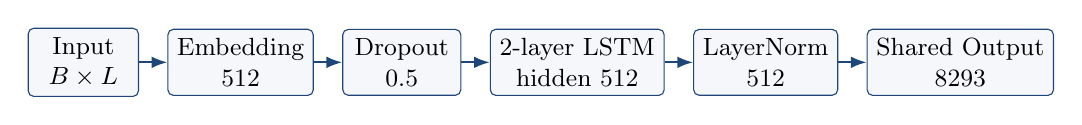
\begin{tikzpicture}[
		layer/.style={draw=ucasblue, fill=lightgray, rounded corners=2pt,
			minimum height=0.8cm, align=center, font=\small},
		arrow/.style={-{Latex[length=2mm]}, thick, draw=ucasblue},
		node distance=0.36cm
	]
		\node[layer, minimum width=1.4cm] (input) {Input\\$B\times L$};
		\node[layer, minimum width=1.8cm, right=of input] (emb) {Embedding\\512};
		\node[layer, minimum width=1.5cm, right=of emb] (drop) {Dropout\\0.5};
		\node[layer, minimum width=1.9cm, right=of drop] (lstm) {2-layer LSTM\\hidden 512};
		\node[layer, minimum width=1.7cm, right=of lstm] (norm) {LayerNorm\\512};
		\node[layer, minimum width=2.0cm, right=of norm] (out) {Shared Output\\8293};
		\foreach \a/\b in {input/emb,emb/drop,drop/lstm,lstm/norm,norm/out}
			\draw[arrow] (\a) -- (\b);
	\end{tikzpicture}
	}

	\vspace{0.55cm}
	\begin{columns}[T,onlytextwidth]
		\begin{column}{0.48\textwidth}
			\begin{block}{上下文建模}
				两层 LSTM 用于学习诗句内部的字符依赖关系，Embedding dropout 和层间 dropout 用于正则化。
			\end{block}
		\end{column}
		\begin{column}{0.48\textwidth}
			\begin{block}{输出层设计}
				输出投影与输入 Embedding 共享权重，只额外学习词表大小的 bias，减少参数并保持表示空间一致。
			\end{block}
		\end{column}
	\end{columns}
\end{frame}

\begin{frame}[fragile]{模型核心代码}
\begin{lstlisting}
class PoetryModel(nn.Module):
    def __init__(self, vocab_size, embedding_dim=512,
                 hidden_dim=512, num_layers=2,
                 dropout=0.5, padding_idx=None):
        super().__init__()
        self.embedding = nn.Embedding(
            vocab_size, embedding_dim, padding_idx=padding_idx
        )
        self.emb_dropout = nn.Dropout(dropout)
        self.lstm = nn.LSTM(
            embedding_dim, hidden_dim,
            num_layers=num_layers,
            batch_first=True,
            dropout=dropout
        )
        self.norm = nn.LayerNorm(hidden_dim)
        self.output_bias = nn.Parameter(torch.zeros(vocab_size))

    def forward(self, x, hidden=None):
        embeds = self.emb_dropout(self.embedding(x))
        output, hidden = self.lstm(embeds, hidden)
        output = self.norm(output)
        output = F.linear(output, self.embedding.weight, self.output_bias)
        return output.reshape(x.size(0) * x.size(1), -1), hidden
\end{lstlisting}
\end{frame}

\begin{frame}{训练配置}
	\begin{columns}[T,onlytextwidth]
		\begin{column}{0.49\textwidth}
			\begin{table}
				\centering
				\small
				\begin{tabular}{l l}
					\toprule
					项目 & 设置 \\
					\midrule
					Batch size & 128 \\
					Epochs & 60 \\
					Embedding dim & 512 \\
					Hidden dim & 512 \\
					LSTM layers & 2 \\
					Dropout & 0.5 \\
					\bottomrule
				\end{tabular}
			\end{table}
		\end{column}
		\begin{column}{0.49\textwidth}
			\begin{table}
				\centering
				\small
				\begin{tabular}{l l}
					\toprule
					项目 & 设置 \\
					\midrule
					Optimizer & AdamW \\
					Learning rate & $1\times10^{-3}$ \\
					Weight decay & $1\times10^{-4}$ \\
					Warmup & 3 epochs \\
					Scheduler & Cosine annealing \\
					Gradient clip & 1.0 \\
					\bottomrule
				\end{tabular}
			\end{table}
		\end{column}
	\end{columns}

	\vspace{0.25cm}
	\begin{block}{评价指标}
		训练和验证阶段记录 loss 与 perplexity，perplexity 定义为 $\mathrm{PPL}=\exp(\mathcal{L})$。
	\end{block}
\end{frame}

\begin{frame}{训练结果}
	\begin{columns}[T,onlytextwidth]
		\begin{column}{0.58\textwidth}
			\begin{table}
				\centering
				\scriptsize
				\begin{tabular}{c c c c c}
					\toprule
					Epoch & Train Loss & Train PPL & Val Loss & Val PPL \\
					\midrule
					1  & 17.1580 & 28289150.5 & 7.2008 & 1340.5 \\
					3  & 6.0091  & 407.1      & 5.7344 & 309.3 \\
					10 & 5.2267  & 186.2      & 5.0532 & 156.5 \\
					20 & 4.9798  & 145.4      & 4.8341 & 125.7 \\
					40 & 4.7265  & 112.9      & 4.6369 & 103.2 \\
					60 & 4.6504  & 104.6      & 4.5867 & 98.2 \\
					\bottomrule
				\end{tabular}
			\end{table}
		\end{column}
		\begin{column}{0.38\textwidth}
			\begin{block}{最终结果}
				\begin{itemize}
					\item 最佳 epoch：60
					\item 验证 loss：4.5867
					\item 验证 PPL：\textbf{98.17}
					\item 梯度范数：0.556
				\end{itemize}
			\end{block}
		\end{column}
	\end{columns}
\end{frame}

\begin{frame}{训练曲线}
	\centering
	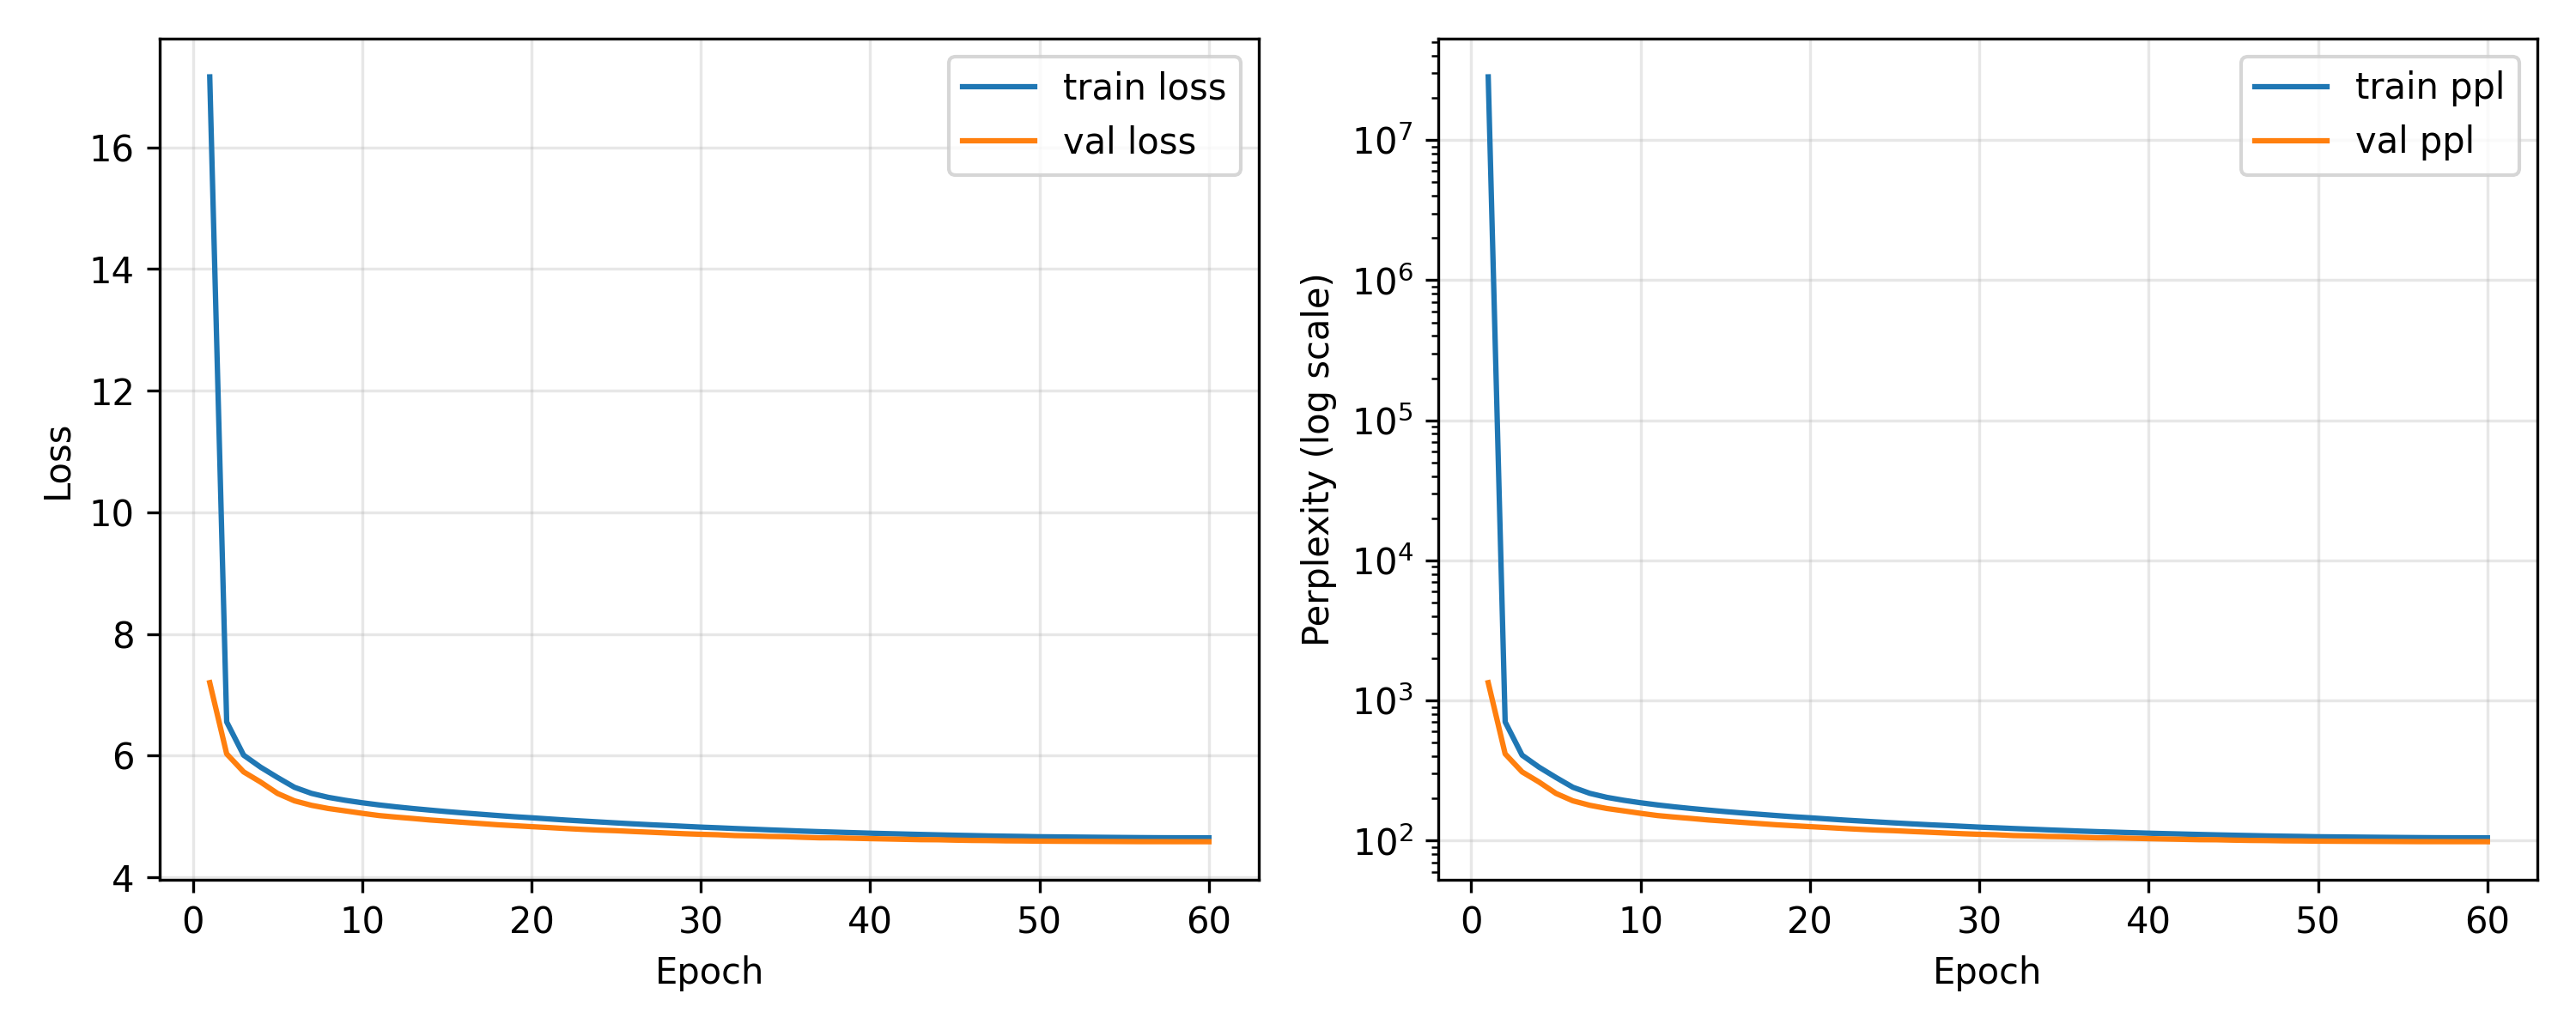
\includegraphics[width=0.88\linewidth]{loss_ppl_curves.png}

	\vspace{0.25cm}
	\begin{itemize}
		\item 前几轮 loss 与 perplexity 快速下降，模型学习到高频字、常见词组和标点模式。
		\item 后期仍缓慢改善，但开放式文本生成存在大量合理后继字符，困惑度不会下降到分类任务那样低。
	\end{itemize}
\end{frame}

\begin{frame}{学习率与梯度范数}
	\centering
	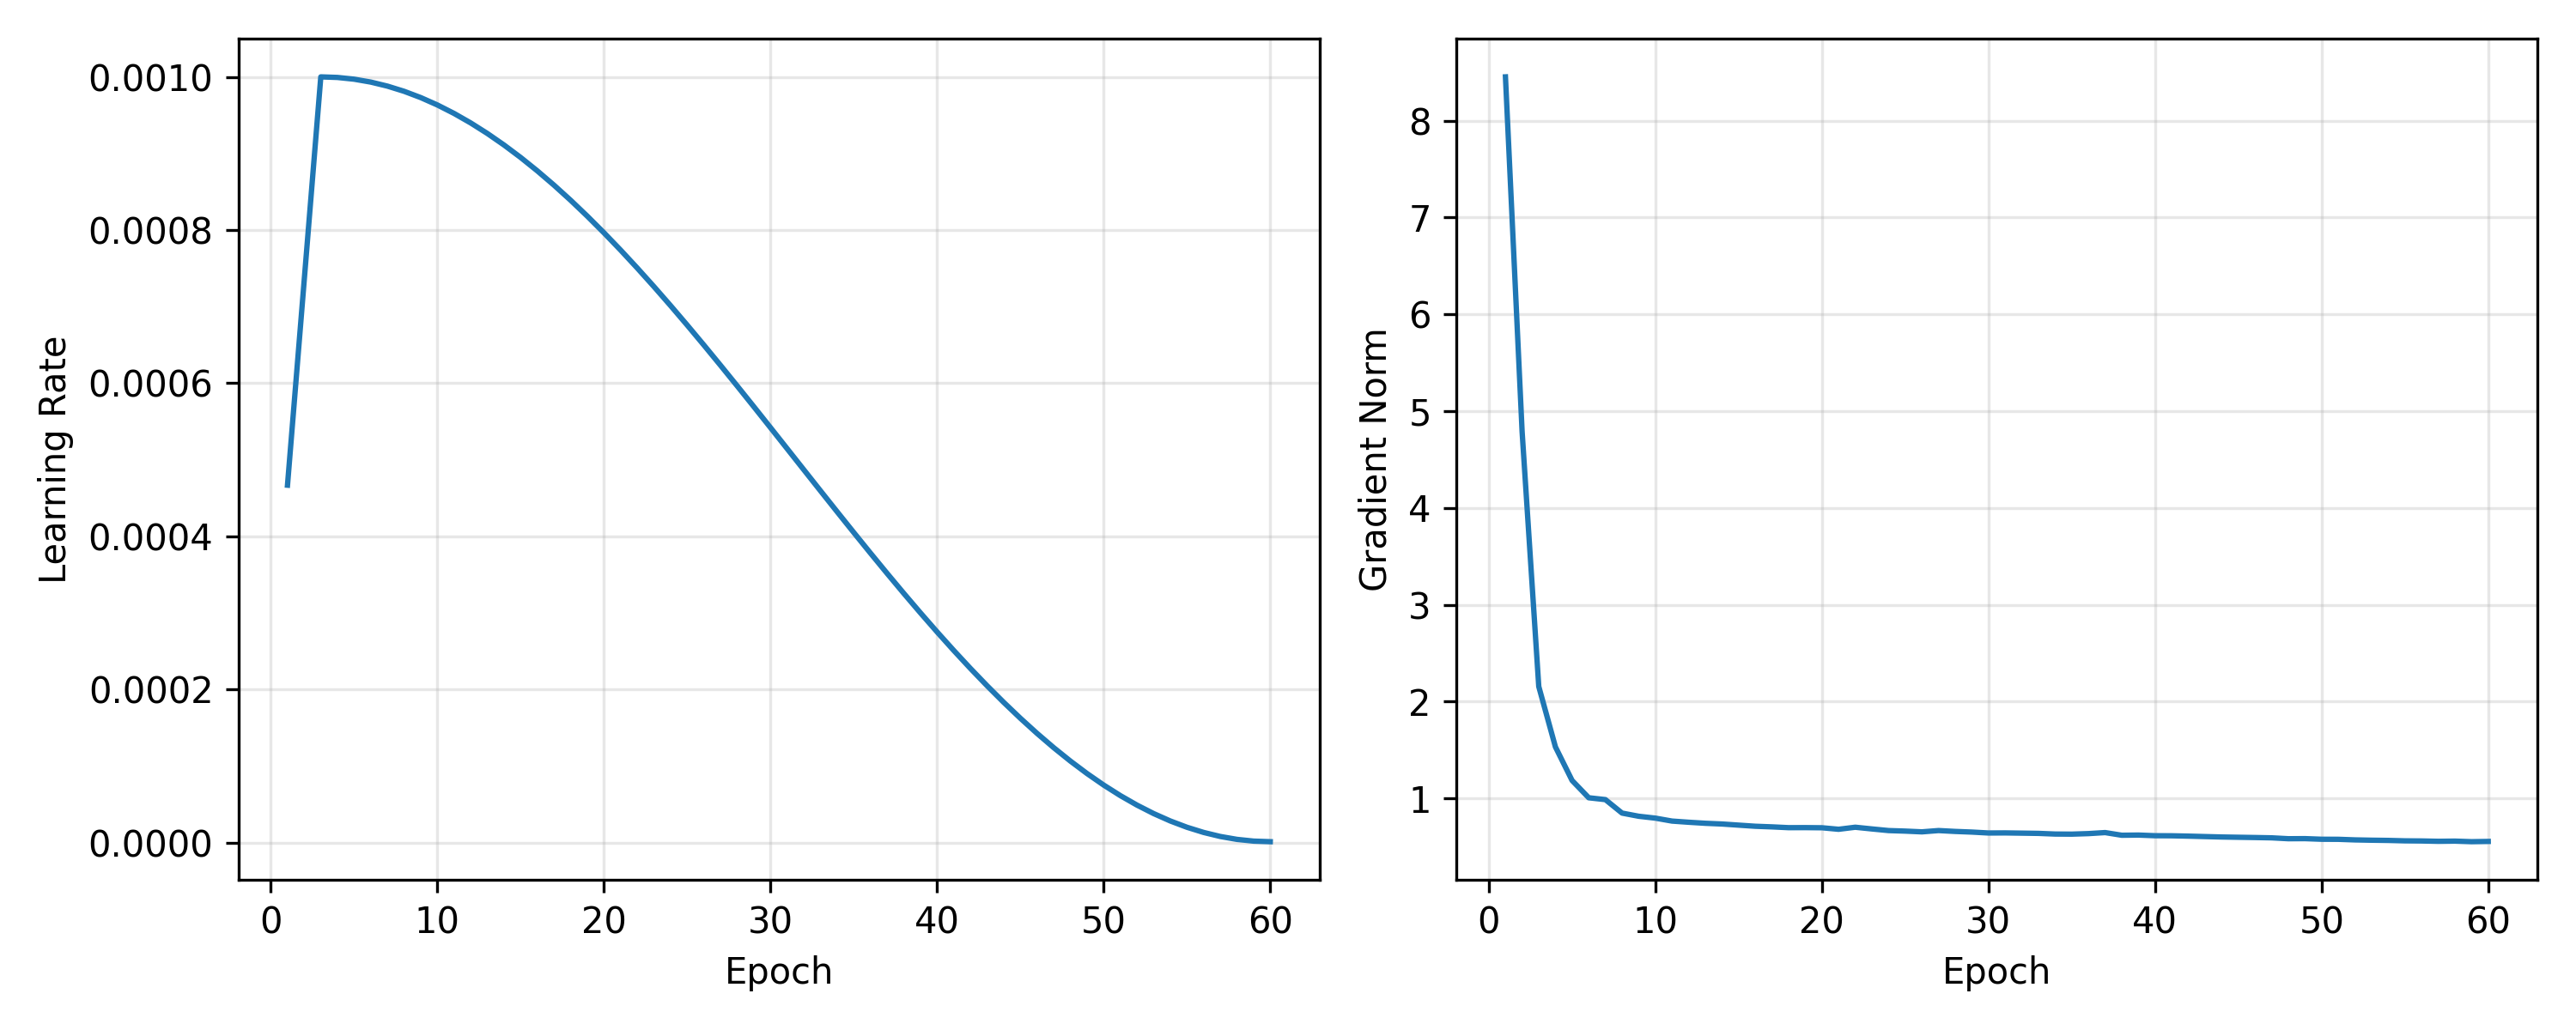
\includegraphics[width=0.88\linewidth]{lr_grad_curves.png}

	\vspace{0.25cm}
	\begin{itemize}
		\item 前 3 轮 warmup 让模型平稳进入训练。
		\item 后续余弦退火逐渐降低学习率，训练后期更新更细。
		\item 梯度范数从第 1 轮的较大值快速下降，说明梯度裁剪和调度策略能控制 RNN 训练不稳定性。
	\end{itemize}
\end{frame}

\begin{frame}{普通续写策略}
	\begin{columns}[T,onlytextwidth]
		\begin{column}{0.47\textwidth}
			\begin{block}{生成流程}
				\begin{enumerate}
					\item 用 \texttt{<START>} 初始化 hidden state
					\item 首句字符逐个强制喂入模型
					\item 首句结束后根据 logits 采样下一个字
					\item 将生成字继续作为下一步输入
				\end{enumerate}
			\end{block}
		\end{column}
		\begin{column}{0.49\textwidth}
			\begin{block}{Top-p 采样}
				按照概率从高到低累积，只保留累计概率不超过 $p$ 的候选集合，再从截断分布中随机采样。
			\end{block}
			\begin{itemize}
				\item temperature = 0.7
				\item top-p = 0.9
				\item 相比 greedy decoding 更不单调
			\end{itemize}
		\end{column}
	\end{columns}
\end{frame}

\begin{frame}{普通续写输出}
	\small
	\poemcard{首句：湖光秋月两相和}{
		湖光秋月两相和，落日江南一半愁。
	}

	\vspace{0.35cm}
	\poemcard{首句：白日依山尽}{
		白日依山尽，青山万里平。天寒云外出，水阔楚山低。流水逢归客，春风入竹林。明朝更惆怅，更寄旧时人。
	}

	\vspace{0.35cm}
	\poemcard{首句：海上生明月}{
		海上生明月，还应忆九天。春风开露叶，玉树含芳菲。今日湖中月，同来旧思君。
	}

	\vspace{0.25cm}
	\begin{itemize}
		\item 局部词组和意象较自然，但长距离主题递进仍然较弱。
	\end{itemize}
\end{frame}

\begin{frame}{藏头诗生成策略}
	\begin{columns}[T,onlytextwidth]
		\begin{column}{0.49\textwidth}
			\begin{block}{为什么要单独设计}
				普通生成允许模型自由决定句长和标点，容易出现一句中间提前生成标点、五言七言长度不稳定等问题。
			\end{block}
			\begin{itemize}
				\item 藏头字必须严格出现在每句首位
				\item 每句需要固定五言或七言长度
				\item 标点位置需要稳定
			\end{itemize}
		\end{column}
		\begin{column}{0.49\textwidth}
			\begin{block}{约束生成方式}
				\begin{itemize}
					\item 每句首字强制喂入藏头字
					\item \texttt{line\_len} 控制五言或七言
					\item 句内屏蔽特殊 token 和标点
					\item 句末手动补 \texttt{，} 或 \texttt{。}
					\item 整首诗共用 hidden state
				\end{itemize}
			\end{block}
		\end{column}
	\end{columns}
\end{frame}

\begin{frame}[fragile]{藏头诗核心逻辑}
\begin{lstlisting}
for i, head in enumerate(heads):
    line = [head]              # 每句首字强制为藏头字
    output, hidden = feed_word(model, word2ix[head], hidden, device)

    for _ in range(line_len - 1):
        next_idx, word = sample_word(output, ix2word, word2ix)
        line.append(word)
        output, hidden = feed_word(model, next_idx, hidden, device)

    punctuation = "。" if i % 2 == 1 or i == len(heads) - 1 else "，"
    line.append(punctuation)
    if punctuation in word2ix:
        _, hidden = feed_word(model, word2ix[punctuation], hidden, device)
\end{lstlisting}

	\vspace{0.25cm}
	\begin{block}{关键点}
		句内不让模型自由生成标点，而是在固定长度后统一补标点，因此格式比普通续写稳定。
	\end{block}
\end{frame}

\begin{frame}{藏头诗输出}
	\begin{columns}[T,onlytextwidth]
		\begin{column}{0.48\textwidth}
			\small
			\poemcard{五言藏头：深度学习}{
				深山幽径可，\\
				度地隔溪深。\\
				学院时时见，\\
				习门声渐闻。
			}

			\vspace{0.25cm}
			\poemcard{七言藏头：丰川祥子}{
				丰年今日在京都，\\
				川路何妨在白云。\\
				祥水自从名不见，\\
				子孙难见好相过。
			}
		\end{column}
		\begin{column}{0.48\textwidth}
			\small
			\poemcard{七言藏头：千早爱音}{
				千里云山万里愁，\\
				早秋城郭旧时秋。\\
				爱君何事君为乐，\\
				音信谁知此意稀。
			}

			\vspace{0.25cm}
			\poemcard{五言藏头：长崎素世}{
				长安风雨老，\\
				崎岖傍空岑。\\
				素彩含长缨，\\
				世上还可怜。
			}
		\end{column}
	\end{columns}
\end{frame}

\begin{frame}{总结}
	\begin{columns}[T,onlytextwidth]
		\begin{column}{0.48\textwidth}
			\begin{block}{完成内容}
				\begin{itemize}
					\item 完成唐诗数据预处理和 DataLoader 构建
					\item 实现两层 LSTM 语言模型
					\item 使用 LayerNorm 与 weight tying 改进输出层
					\item 记录训练 loss、PPL、学习率和梯度范数
					\item 实现普通续写与藏头诗生成
				\end{itemize}
			\end{block}
		\end{column}
		\begin{column}{0.48\textwidth}
			\begin{block}{后续改进}
				\begin{itemize}
					\item 加入重复惩罚，减少常见意象反复组合
					\item 在解码阶段加入韵脚约束
					\item 尝试更强的序列模型或预训练语言模型
					\item 进一步提升整首诗的主题连贯性
				\end{itemize}
			\end{block}
		\end{column}
	\end{columns}
\end{frame}

\end{document}
